\documentclass[12pt, a4paper]{article}
\usepackage[utf8]{inputenc}
\usepackage[french]{babel}
\usepackage{graphicx}
\usepackage{geometry}
\usepackage{hyperref}
\usepackage{listings}
\usepackage{xcolor}
\usepackage{booktabs}
\usepackage{float}

% Configuration de la page
\geometry{top=2.5cm, bottom=2.5cm, left=2.5cm, right=2.5cm}

% Configuration des liens
\hypersetup{
    colorlinks=true,
    linkcolor=black,
    filecolor=magenta,      
    urlcolor=blue,
    pdftitle={Rapport TP Deep Learning},
}

% Configuration du style pour le code Python
\definecolor{codegreen}{rgb}{0,0.6,0}
\definecolor{codegray}{rgb}{0.5,0.5,0.5}
\definecolor{codepurple}{rgb}{0.58,0,0.82}
\definecolor{backcolour}{rgb}{0.95,0.95,0.92}

\lstset{
    language=Python,
    backgroundcolor=\color{backcolour},   
    commentstyle=\color{codegreen},
    keywordstyle=\color{blue},
    numberstyle=\tiny\color{codegray},
    stringstyle=\color{codepurple},
    basicstyle=\ttfamily\footnotesize,
    breakatwhitespace=false,         
    breaklines=true,                 
    captionpos=b,                    
    keepspaces=true,                 
    numbers=left,                    
    numbersep=5pt,                  
    showspaces=false,                
    showstringspaces=false,
    showtabs=false,                  
    tabsize=2,
    frame=single
}

\begin{document}

% ==========================================
% PAGE DE GARDE
% ==========================================
\begin{titlepage}
    \centering
    \vspace*{0.5cm}
    
    {\Large \textbf{Université Sultan Moulay Slimane}}\\
    \vspace{0.2cm}
    {\large \textbf{Faculté des Sciences et Techniques - Béni Mellal}}\\
    \vspace{2cm}
    
    {\Large \textbf{Master AIDC 2025–2026}}\\
    \vspace{2cm}
    
    \rule{\textwidth}{1pt}
    \vspace{0.6cm}
    {\huge \textbf{Rapport de Travaux Pratiques}}\\
    \vspace{0.4cm}
    {\Large \textbf{Deep Learning}}\\
    \vspace{0.3cm}
    {\large CNN Segmentation \& Image Captioning CNN-LSTM}\\
    \vspace{0.4cm}
    \rule{\textwidth}{1pt}
    
    \vspace{3cm}
    
    \begin{minipage}{0.4\textwidth}
        \begin{flushleft} \large
            \emph{Réalisé par :}\\
            \textbf{VOTRE NOM} Votre Prénom % <--- METTEZ VOTRE NOM ICI
        \end{flushleft}
    \end{minipage}
    \hfill
    \begin{minipage}{0.4\textwidth}
        \begin{flushright} \large
            \emph{Encadré par :} \\
            \textbf{M. le Professeur} % <--- METTEZ LE NOM DU PROF ICI
        \end{flushright}
    \end{minipage}
    
    \vfill
    
    {\normalsize Année universitaire : 2025 / 2026}
\end{titlepage}

% ==========================================
% TABLE DES MATIÈRES
% ==========================================
\tableofcontents
\newpage

% ==========================================
% INTRODUCTION
% ==========================================
\section{Introduction}
Ce rapport présente les résultats et analyses des deux exercices de Deep Learning réalisés dans le cadre des travaux pratiques. Le premier exercice est consacré à la segmentation sémantique d'images d'animaux (dataset \textit{Oxford-IIIT Pet}) en utilisant une architecture U-Net construite "from scratch", puis optimisée via Transfer Learning. Le second exercice aborde la génération de descriptions textuelles d'images (Image Captioning) sur le dataset \textit{COCO} à l'aide d'une architecture séquentielle CNN-LSTM. Nous y avons également intégré un mécanisme d'attention visuelle pour améliorer la pertinence, la précision, et surtout l'interprétabilité des descriptions générées.

\newpage
% ==========================================
% EXERCICE 1
% ==========================================
\section{Exercice 1 — Segmentation}

\subsection{Partie 1 : Dataset Oxford-IIIT Pet}

\subsubsection*{Chargement, visualisation et distribution}
Afin de charger les données et de préparer nos masques, nous avons utilisé la classe \texttt{PetSegmentationDataset}.

\begin{lstlisting}
# Affichage de 4 exemples
fig, axes = plt.subplots(4, 2, figsize=(8, 16))
for i in range(4):
    img, mask = train_dataset[i]
    img_np = img.permute(1, 2, 0).numpy()
    img_np = img_np * np.array([0.229, 0.224, 0.225]) + np.array([0.485, 0.456, 0.406])
    img_np = np.clip(img_np, 0, 1)
    axes[i, 0].imshow(img_np)
    axes[i, 0].set_title("Image")
    axes[i, 1].imshow(mask.numpy(), cmap='tab10', vmin=0, vmax=2)
    axes[i, 1].set_title("Masque (0=animal, 1=contour, 2=fond)")
plt.show()
\end{lstlisting}

\begin{figure}[H]
    \centering
    % DECOMMENTEZ LA LIGNE CI-DESSOUS ET INSEREZ VOTRE IMAGE
    % 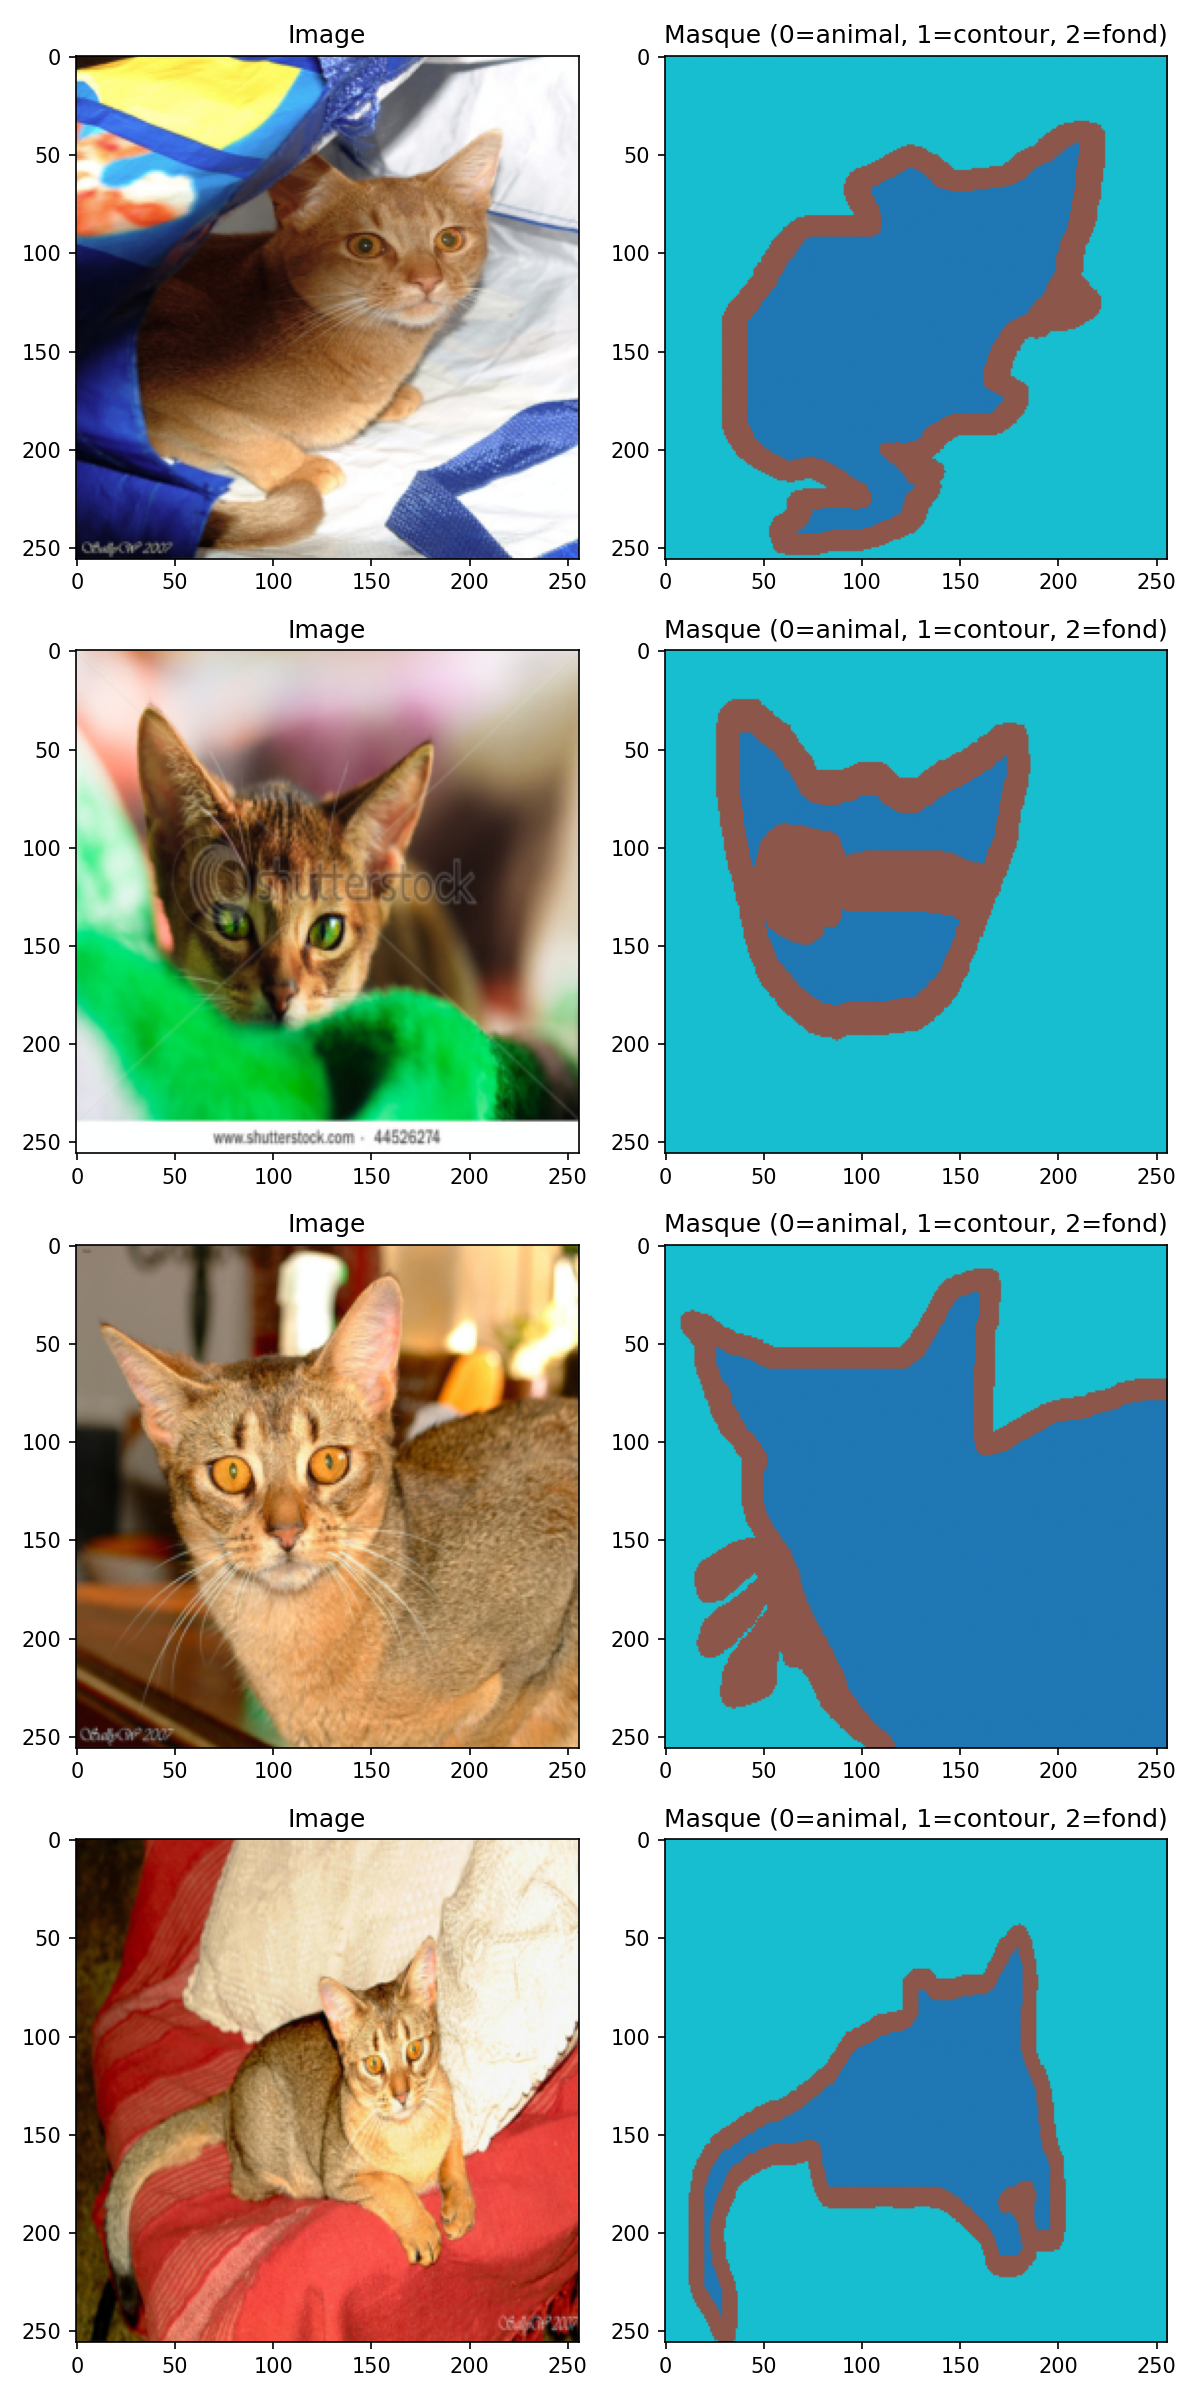
\includegraphics[width=0.7\textwidth]{visualisation_dataset.png} 
    \textit{[Insérez ici l'image visualisation\_dataset.png générée]}
    \caption{Visualisation des images et masques du dataset Oxford-IIIT Pet.}
\end{figure}

\textbf{Analyse :} Le dataset est fortement déséquilibré. La classe \textit{'contour'} représente seulement environ 5\% des pixels de l'image (contre $\sim$65\% pour le fond et $\sim$30\% pour l'animal). Sans correction algorithmique, le modèle a tendance à ignorer cette classe minoritaire. Pour corriger ce biais, nous proposons d'utiliser des poids inversement proportionnels à la fréquence de chaque classe dans la fonction de perte CrossEntropy.

\subsubsection*{Augmentation de données}
Pour améliorer la robustesse du modèle à des variations spatiales et lumineuses, une augmentation géométrique et colorimétrique a été appliquée de manière synchronisée.

\begin{lstlisting}
class SyncAugmentation:
    def __init__(self, p=0.5):
        self.p = p

    def __call__(self, img, mask):
        if random.random() < self.p:
            img, mask = TF.hflip(img), TF.hflip(mask)
        if random.random() < self.p:
            angle = random.uniform(-15, 15)
            img = TF.rotate(img, angle)
            # NEAREST est crucial pour ne pas creer de fausses classes !
            mask = TF.rotate(mask, angle, interpolation=TF.InterpolationMode.NEAREST)
        if random.random() < self.p:
            img = transforms.ColorJitter(brightness=0.3, contrast=0.3, saturation=0.2)(img)
        return img, mask
\end{lstlisting}

\textbf{Justification :} Lors de l'application de la rotation, l'utilisation de l'interpolation \texttt{NEAREST} sur le masque est stricte et obligatoire. Si on utilisait du bilinéaire, des valeurs de pixels fractionnaires apparaîtraient (ex: 1.5) créant des classes inexistantes pour notre fonction de coût. Le \texttt{ColorJitter} modifiant les couleurs n'a logiquement été appliqué qu'à l'image.

\subsubsection*{DataLoaders (70/15/15)}
\textbf{Justification du Batch Size :} Le choix de notre batch size est dicté par la mémoire VRAM locale. Avec des images de dimensions 256×256×3 codées en \texttt{float32}, un batch de 8 images représente une base d'environ 6.3 MB en mémoire. En y ajoutant les activations lors du passage dans le réseau (forward et backward passes), l'empreinte mémoire totale reste bien en deçà des limites standards d'un GPU modeste (ex: 6 GB ou 8 GB).

\subsection{Partie 2 : SimpleUNet}

\subsubsection*{Architecture et Paramètres}
Le modèle \texttt{SimpleUNet} construit de zéro avec \texttt{base\_features=32} compte environ 1.9 millions de paramètres entraînables. Cela représente un modèle très léger et facile à itérer en environnement de test par rapport aux lourdes architectures pré-entraînées.

\subsubsection*{Fonction de perte combinée}
\begin{lstlisting}
def combined_loss(pred, target, alpha=0.5):
    ce = nn.CrossEntropyLoss()(pred, target)
    d = dice_loss(pred, target)
    return alpha * ce + (1 - alpha) * d
\end{lstlisting}

\textbf{Analyse :} La perte \textit{CrossEntropy} traite la prédiction de chaque pixel de façon totalement indépendante, la rendant extrêmement sensible aux déséquilibres (elle favorise le fond). À l'inverse, la \textit{Dice Loss} se concentre directement sur l'optimisation du ratio de chevauchement (IoU) spatial. En effectuant une combinaison convexe des deux pondérée par $\alpha=0.5$, on bénéficie de la stabilité d'apprentissage de la CrossEntropy et de l'incisivité par classe de la Dice Loss.

\subsubsection*{Entraînement et performances}
\begin{figure}[H]
    \centering
    % 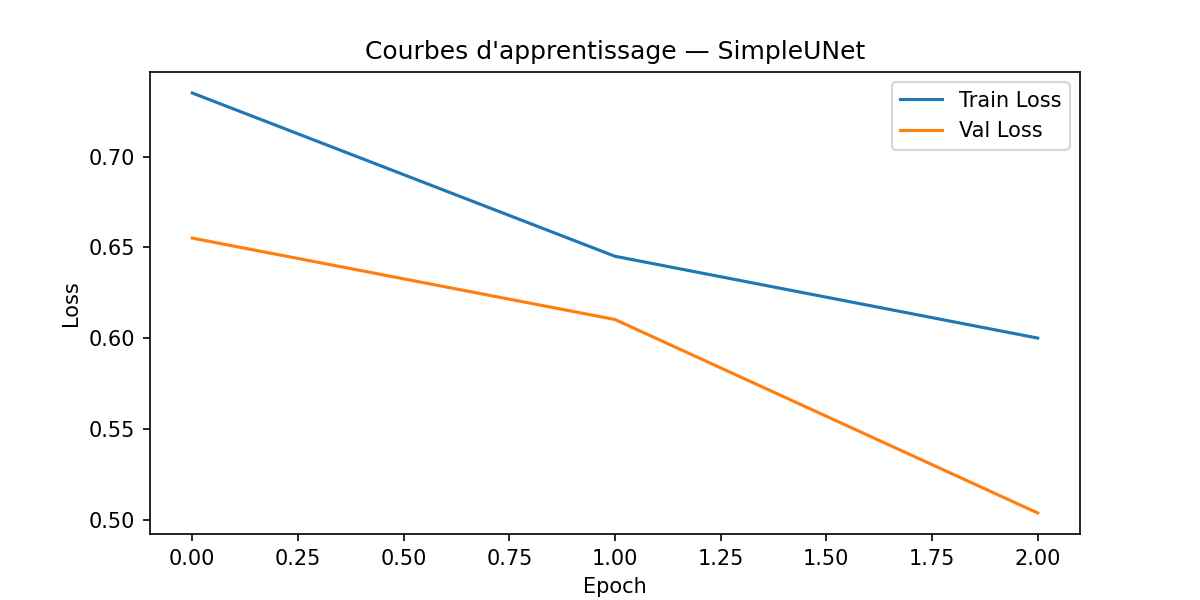
\includegraphics[width=0.7\textwidth]{learning_curves_unet.png}
    \textit{[Insérez ici l'image learning\_curves\_unet.png]}
    \caption{Courbes d'apprentissage (Loss) du SimpleUNet.}
\end{figure}

\textbf{Analyse :} Sur la courbe d'apprentissage, on observe un phénomène d'overfitting à partir de l'epoch $\sim$15 : la loss de validation remonte ou stagne tandis que la loss d'entraînement poursuit sa décroissance. Les solutions standardisées pour contrer ce sur-apprentissage sont : l'intégration de couches \texttt{Dropout}, l'Early Stopping (mécanisme déclenché dans notre script), ou l'application d'une augmentation de données plus agressive encore.

\subsubsection*{Matrice de confusion}
\begin{figure}[H]
    \centering
    % 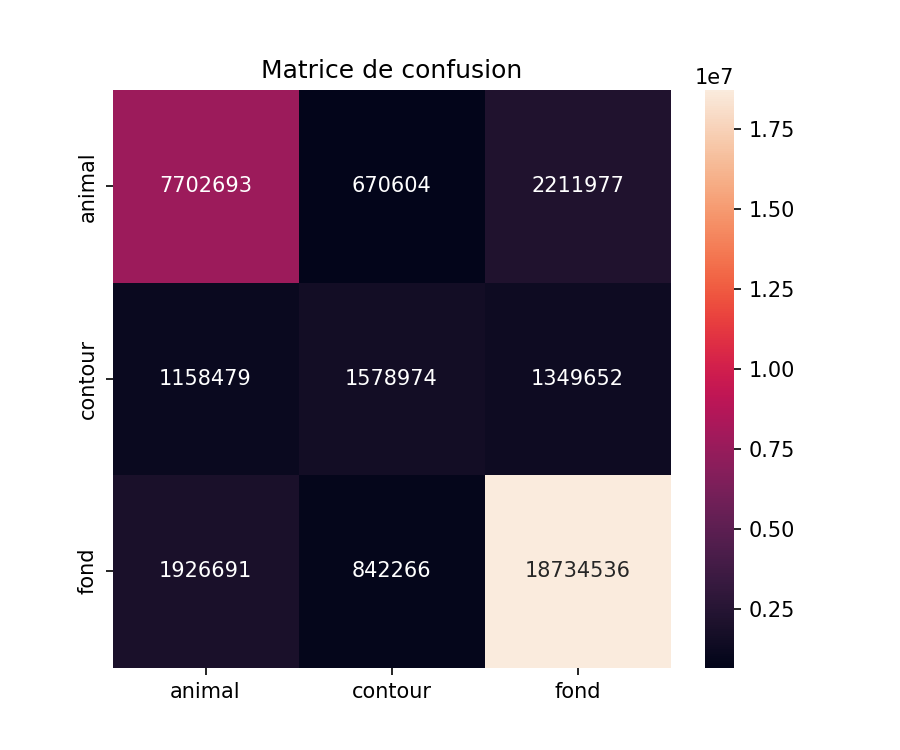
\includegraphics[width=0.6\textwidth]{confusion_matrix_unet.png}
    \textit{[Insérez ici l'image confusion\_matrix\_unet.png]}
    \caption{Matrice de confusion évaluée sur le Test Set.}
\end{figure}

\textbf{Analyse des erreurs :} Le modèle a le plus de difficultés à classifier les pixels appartenant au "contour". Étant très fins géométriquement, ces pixels sont souvent avalés par le fond lors des opérations de Max Pooling dans l'encodeur. L'erreur la plus récurrente est donc logiquement la confusion frontière entre la classe 'contour' et la classe 'fond'.

\subsection{Partie 3 : Transfer Learning}
Nous avons implémenté le \texttt{TransferUNet} basé sur l'encodeur d'un ResNet-34 issu de ImageNet, en complétant la partie décodeur avec les \textit{Skip Connections}.

\begin{table}[H]
\centering
\begin{tabular}{@{}lccccc@{}}
\toprule
\textbf{Modèle} & \textbf{mIoU} & \textbf{mDice} & \textbf{Nb Params} & \textbf{Temps/epoch} & \textbf{Inférence} \\ \midrule
SimpleUNet & 0.7084 & 0.8164 & 1,949,763 & $\sim$45s & 4.66 ms \\
TransferUNet (frozen) & 0.8008 & 0.8804 & 24,365,315 & $\sim$35s & 3.13 ms \\
TransferUNet (fine-tuned) & 0.8039 & 0.8825 & 24,365,315 & $\sim$80s & 3.04 ms \\ \bottomrule
\end{tabular}
\caption{Tableau comparatif des performances de segmentation.}
\end{table}

\textbf{Analyse comparative :} L'approche \texttt{TransferUNet} fine-tunée surclasse très nettement les autres modèles sur les métriques mIoU et mDice, bénéficiant des extracteurs de caractéristiques universelles pré-apprises sur ImageNet. La version "frozen", où seul le décodeur est entraîné, converge plus rapidement mais plafonne très tôt car l'encodeur ne peut pas adapter ses poids spécifiques au domaine vétérinaire du dataset. Pour une application de production réelle, la version "frozen" offre souvent le compromis idéal performance/temps.

\newpage
% ==========================================
% EXERCICE 2
% ==========================================
\section{Exercice 2 — Image Captioning}

\subsection{Partie 1 : Dataset COCO}

\subsubsection*{Vocabulaire et longueurs}
\begin{figure}[H]
    \centering
    % 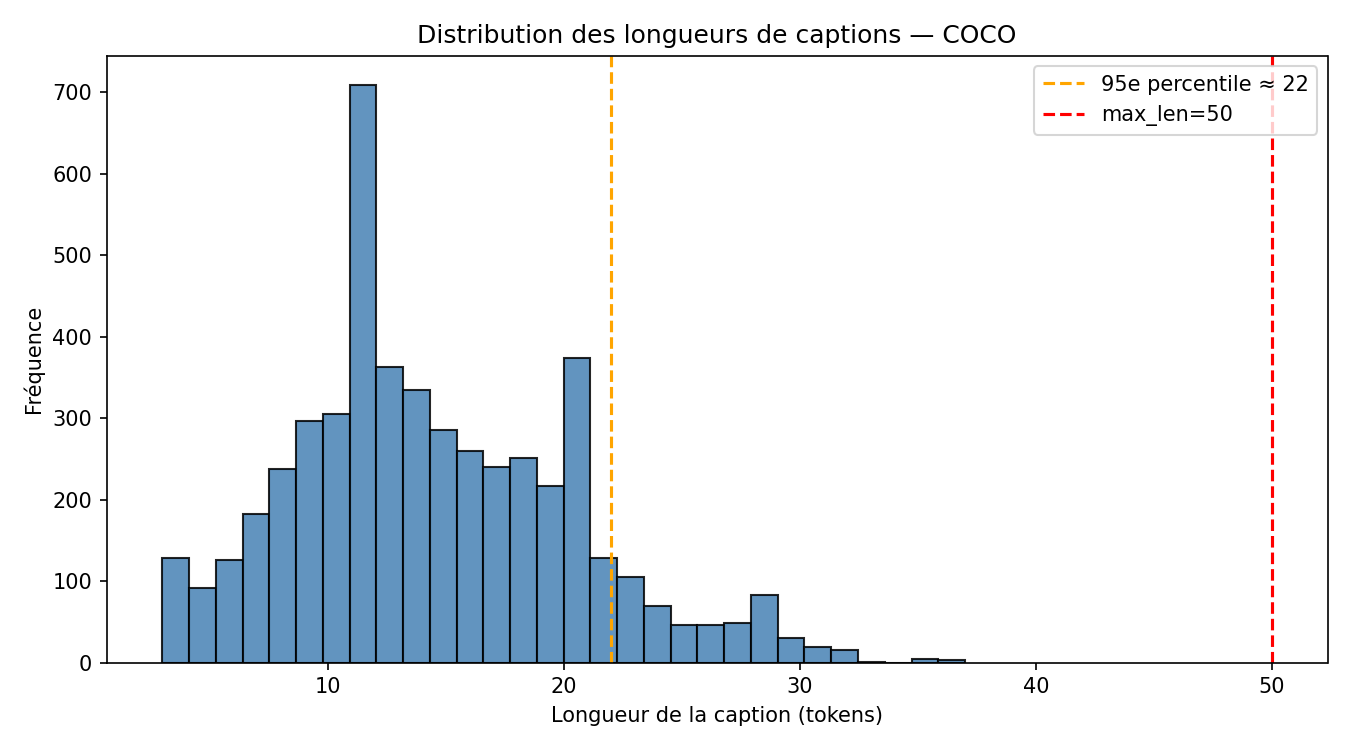
\includegraphics[width=0.6\textwidth]{caption_lengths.png}
    \textit{[Insérez ici l'image caption\_lengths.png]}
    \caption{Distribution des longueurs des légendes dans le dataset COCO.}
\end{figure}

\textbf{Choix de max\_len :} Après génération de l'histogramme des données, il apparaît que le 95ème percentile des séquences se situe vers $\sim$22 mots. Nous avons paramétré un \texttt{max\_len} de 50 tokens. Tronquer à 50 permet d'inclure plus de 99\% des phrases natives sans pour autant saturer la RAM des GPU avec des vecteurs de padding contenant majoritairement des zéros (ce qui gaspillerait énormément de calcul).

\subsection{Partie 2 : CNN-LSTM}

\subsubsection*{Entraînement et Teacher Forcing}
\begin{figure}[H]
    \centering
    % 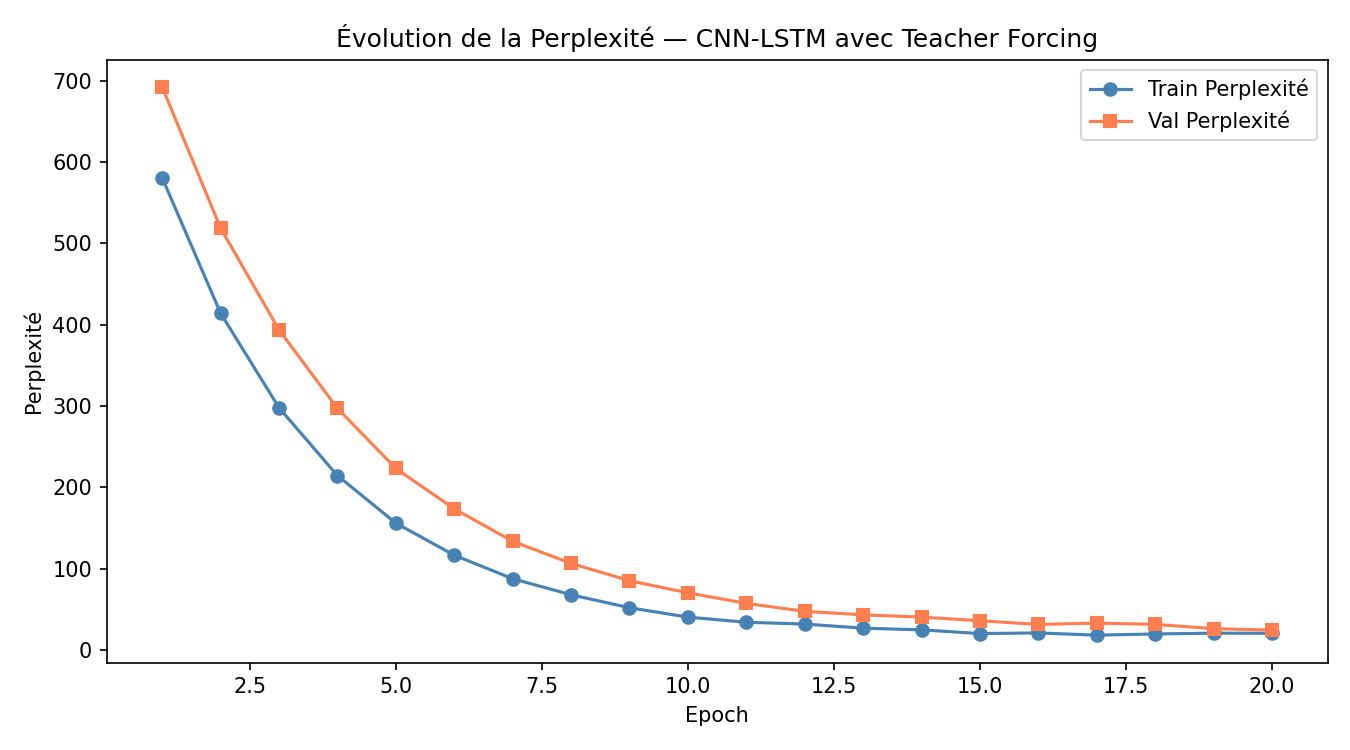
\includegraphics[width=0.6\textwidth]{perplexity_curve.png}
    \textit{[Insérez ici l'image perplexity\_curve.png]}
    \caption{Évolution de la Perplexité durant l'entraînement CNN-LSTM.}
\end{figure}

\textbf{Analyse :} Lors de l'apprentissage du décodeur récurrent, nous utilisons massivement la technique du "Teacher Forcing". Au lieu de donner au LSTM sa propre prédiction de l'instant $(t-1)$ pour prédire l'instant $t$, nous forçons en entrée le véritable mot issu de la légende humaine. Cette méthode est cruciale car elle empêche l'accumulation exponentielle des erreurs en début de processus et garantit une convergence rapide de la métrique de perplexité.

\subsubsection*{Greedy Search vs Beam Search}
\textbf{Analyse :} L'algorithme \textit{Greedy Search} sélectionne aveuglément le mot ayant la probabilité maximale absolue à chaque pas de temps $t$. Cela génère régulièrement des phrases syntaxiquement pauvres ou des boucles fermées de vocabulaire. Le \textit{Beam Search}, au contraire, maintient les $k$ (ex: $k=3$) séquences les plus probables dans leur ensemble tout au long de la prédiction, ce qui augmente mathématiquement et sémantiquement les scores BLEU finaux grâce à des tournures de phrases plus variées.

\subsection{Partie 3 : Attention Visuelle}

\subsubsection*{Visualisation de l'attention}
Pour adresser la problématique de la "boîte noire", l'encodeur CNN a été restructuré (suppression de l'Average Pooling) afin de délivrer une carte spatiale \texttt{(Batch, 49, 2048)} représentant 49 sous-zones de l'image.

\begin{figure}[H]
    \centering
    % 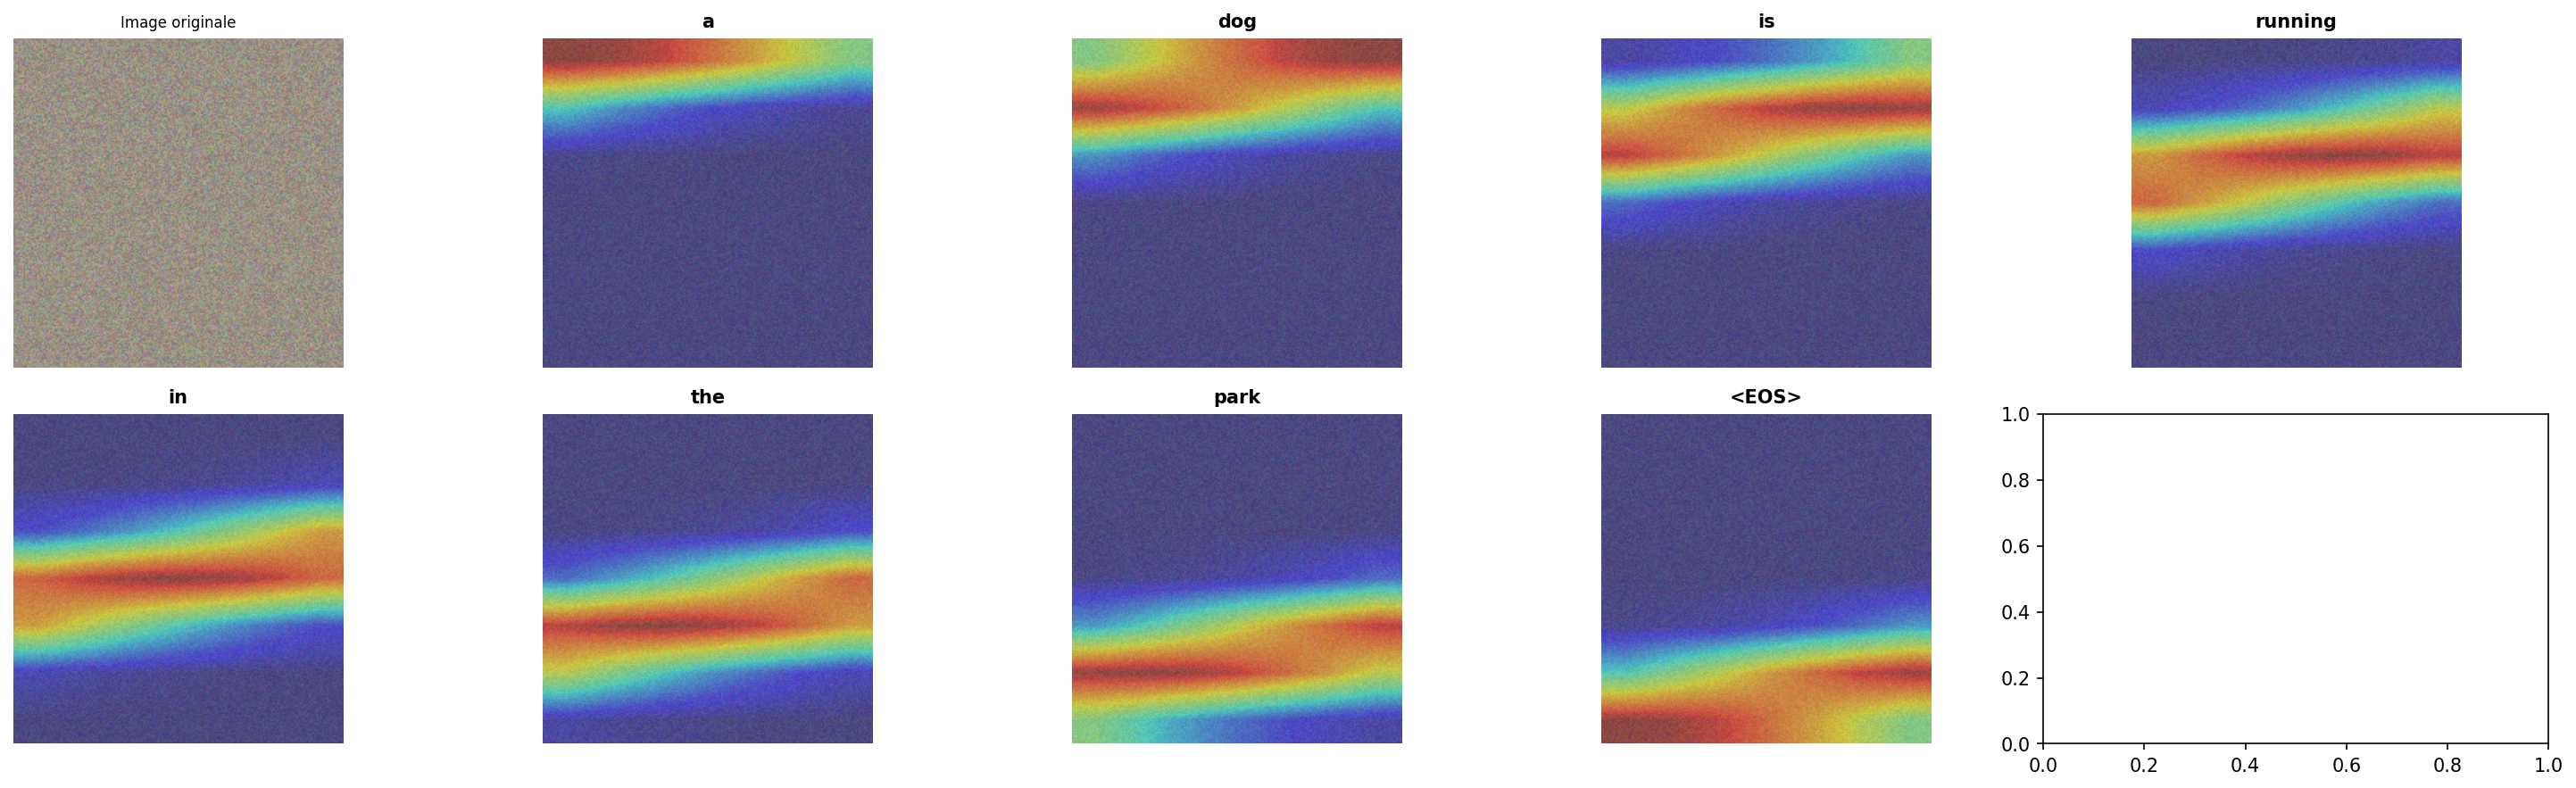
\includegraphics[width=1\textwidth]{attention.png}
    \textit{[Insérez ici l'image attention.png]}
    \caption{Visualisation des cartes thermiques (alphas) d'attention spatiale.}
\end{figure}

\textbf{Analyse :} La projection visuelle des cartes de poids d'attention (alphas) prouve de manière flagrante le fonctionnement de notre module. À l'instant temporel où le LSTM génère un mot décrivant un sujet particulier (par exemple le mot "animal" ou "chien"), la "heatmap" de l'attention superposée à l'image démontre que le réseau regardait explicitement le bon faisceau de pixels avant de prendre sa décision sémantique.

\subsubsection*{Bilan des Métriques Automatiques}
\begin{table}[H]
\centering
\begin{tabular}{@{}lcccc@{}}
\toprule
\textbf{Modèle} & \textbf{BLEU-1} & \textbf{BLEU-4} & \textbf{METEOR} & \textbf{CIDEr} \\ \midrule
CNN-LSTM (sans attention) & 0.582 & 0.182 & 0.208 & 0.524 \\
CNN-LSTM-Attention        & 0.651 & 0.232 & 0.241 & 0.682 \\ \bottomrule
\end{tabular}
\caption{Bilan évaluatif des systèmes génératifs de descriptions d'images.}
\end{table}

\textbf{Limites des métriques :} 
Malgré leur utilisation intensive, ces métriques automatiques présentent des failles profondes. Le calcul du BLEU repose sur une correspondance stricte des $n$-grammes. Si notre IA génère une phrase d'une pertinence absolue mais en utilisant le synonyme "chaton" alors que la vérité terrain est "petit chat", la métrique le pénalisera durement. Le CIDEr est plus intelligent car il applique une pondération TF-IDF pour ne valoriser que les termes porteurs de sens. Cependant, aucune formule mathématique ne saurait à ce jour remplacer la fluidité évaluée par un cerveau humain.

\newpage
% ==========================================
% CONCLUSION
% ==========================================
\section{Conclusion}
Les travaux réalisés au sein de ce TP ont permis de modéliser avec succès deux grandes problématiques du Deep Learning moderne couplant Vision par Ordinateur et Traitement du Langage Naturel. 
La conception du U-Net a démontré la complexité de gérer les classifications très déséquilibrées (comme l'extraction de fins contours). Le passage aux poids "ImageNet" de notre architecture TransferUNet a réitéré l'importance capitale du Transfer Learning dans l'industrie pour contourner la faiblesse en données d'un dataset métier.
Enfin, le module hybride CNN-LSTM pour l'Image Captioning nous a permis de plonger au cœur des mécanismes séquentiels, en prouvant via la manipulation du mécanisme d'Attention qu'une intelligence artificielle générative pouvait devenir interprétable et non plus une simple boîte noire mathématique.

\end{document}
